\documentclass{article}
\usepackage{listings}
\usepackage{booktabs}
\usepackage{here}
\usepackage{subcaption}
\usepackage{tikz}
\usepackage{amsmath}
\usepackage{graphicx}
\usepackage[colorlinks=true, allcolors=black]{hyperref}

% Set page size and margins
\usepackage[letterpaper,top=2cm,bottom=2cm,left=3cm,right=3cm,marginparwidth=1.75cm]{geometry}

% % Remove section numbering
% \renewcommand{\thesection}{}
% \renewcommand{\thesubsection}{}

% \newcommand{\code}[1]{{\tt #1}}
% \newcommand\blankpage{%
% 	\null
% 	\thispagestyle{empty}%
% 	\addtocounter{page}{-1}%
% 	\newpage}


%%%% Define style for code %%%%
\lstdefinestyle{mystyle}{
    language=Java,
	numbers=left,
    basicstyle=\ttfamily\footnotesize,
    keywordstyle=\color{blue},
    commentstyle=\color{gray},
    stringstyle=\color{brown},
    showstringspaces=false,
    breaklines=true,
    frame=single, % Aggiunge il bordo
    frameround=tttt, % Angoli arrotondati
    backgroundcolor=\color{lightgray!20}, % Sfondo leggermente grigio
    rulecolor=\color{black}, % Colore del bordo
}
\lstset{style=mystyle} % stile definito come default
\captionsetup[lstlisting]{labelformat=empty} % Disable listing numbering
%%%%%%%%%%%%%%%%%%%%%%%%%%%%%%

\newcommand{\codepath}{../app/src/main/java/com/example/stepappv4}


\title{
	\normalfont\normalsize
	\textsc{Mobile and Wearable Computing SA 2024-2025\\%
	Universit\`a della Svizzera italiana}\\
	\vspace{25pt}
	\rule{\linewidth}{0.5pt}\\
	\vspace{20pt}
	{\huge Assignment 2}\\
	\vspace{12pt}
	\rule{\linewidth}{1pt}\\
	\vspace{12pt}
}

\author{
  Paolo Deidda \\
  \text{paolo.deidda@usi.ch} \\ 
  \url{https://github.com/USI-Projects-Collection/MWCTutorial04.git}
}


\begin{document}
\maketitle

\tableofcontents

\section*{Important notes}
asdfasdf

\newpage
\section{Exercise 1 – Android Basics}

\begin{enumerate}
    \item  \textbf{What does the \texttt{android:minSdkVersion} in an Android project indicate?}

    The \texttt{android:minSdkVersion} attribute specifies the minimum Android OS version that the app can run on. It ensures that the app will only be installable on devices with an OS version \textit{equal to or higher} than the declared version. For example, if \texttt{minSdkVersion} is set to 21, the app will only work on devices running Android 5.0 (Lollipop) or newer.
    \\
    
    \item \textbf{Why does Android documentation indicate that declaring the attribute \texttt{android:\\maxSdkVersion} is not recommended?}

    The Android documentation advises against using \texttt{maxSdkVersion} because it restricts the app's availability for future Android versions. If this attribute is set, the app won't be available for users running newer versions of Android, even if it could still work. This can cause compatibility and distribution issues as new Android versions are released.
    \\
    
    \item \textbf{What are the two types of Navigation Drawer? Explain the differences between the two types.}

    There are two types of Navigation Drawer in Android:
    \begin{itemize}
        \item \textbf{Permanent Navigation Drawer}: This type is always visible alongside the app's content, often used in tablet layouts or on large screens. The main content of the app is displayed next to the drawer.
        \item \textbf{Modal Navigation Drawer}: This type is hidden by default and slides in over the app's content when triggered. It is commonly used in mobile apps where screen space is limited.
    \end{itemize}
    

    \textbf{Differences:} The permanent drawer is better suited for larger screens where space is not an issue, while the modal drawer is more suitable for smaller screens, as it saves space by presenting the drawer as an overlay.
\end{enumerate}

\newpage
\section{Exercise 2 – Material Design}
    
    \subsection{Change App Icon}
        To change our app's icon, I used Android Studio's built-in feature to generate icons (see Figure~\ref{fig:ex2_1.1}). I navigated to the \texttt{res} folder, right-clicked on the \texttt{drawable} folder, and selected \textit{New} $\rightarrow$ \textit{Image Asset}. After selecting the image I had previously imported, Android Studio automatically generated the required icons.
        
        \begin{figure}[H]
            \centering
            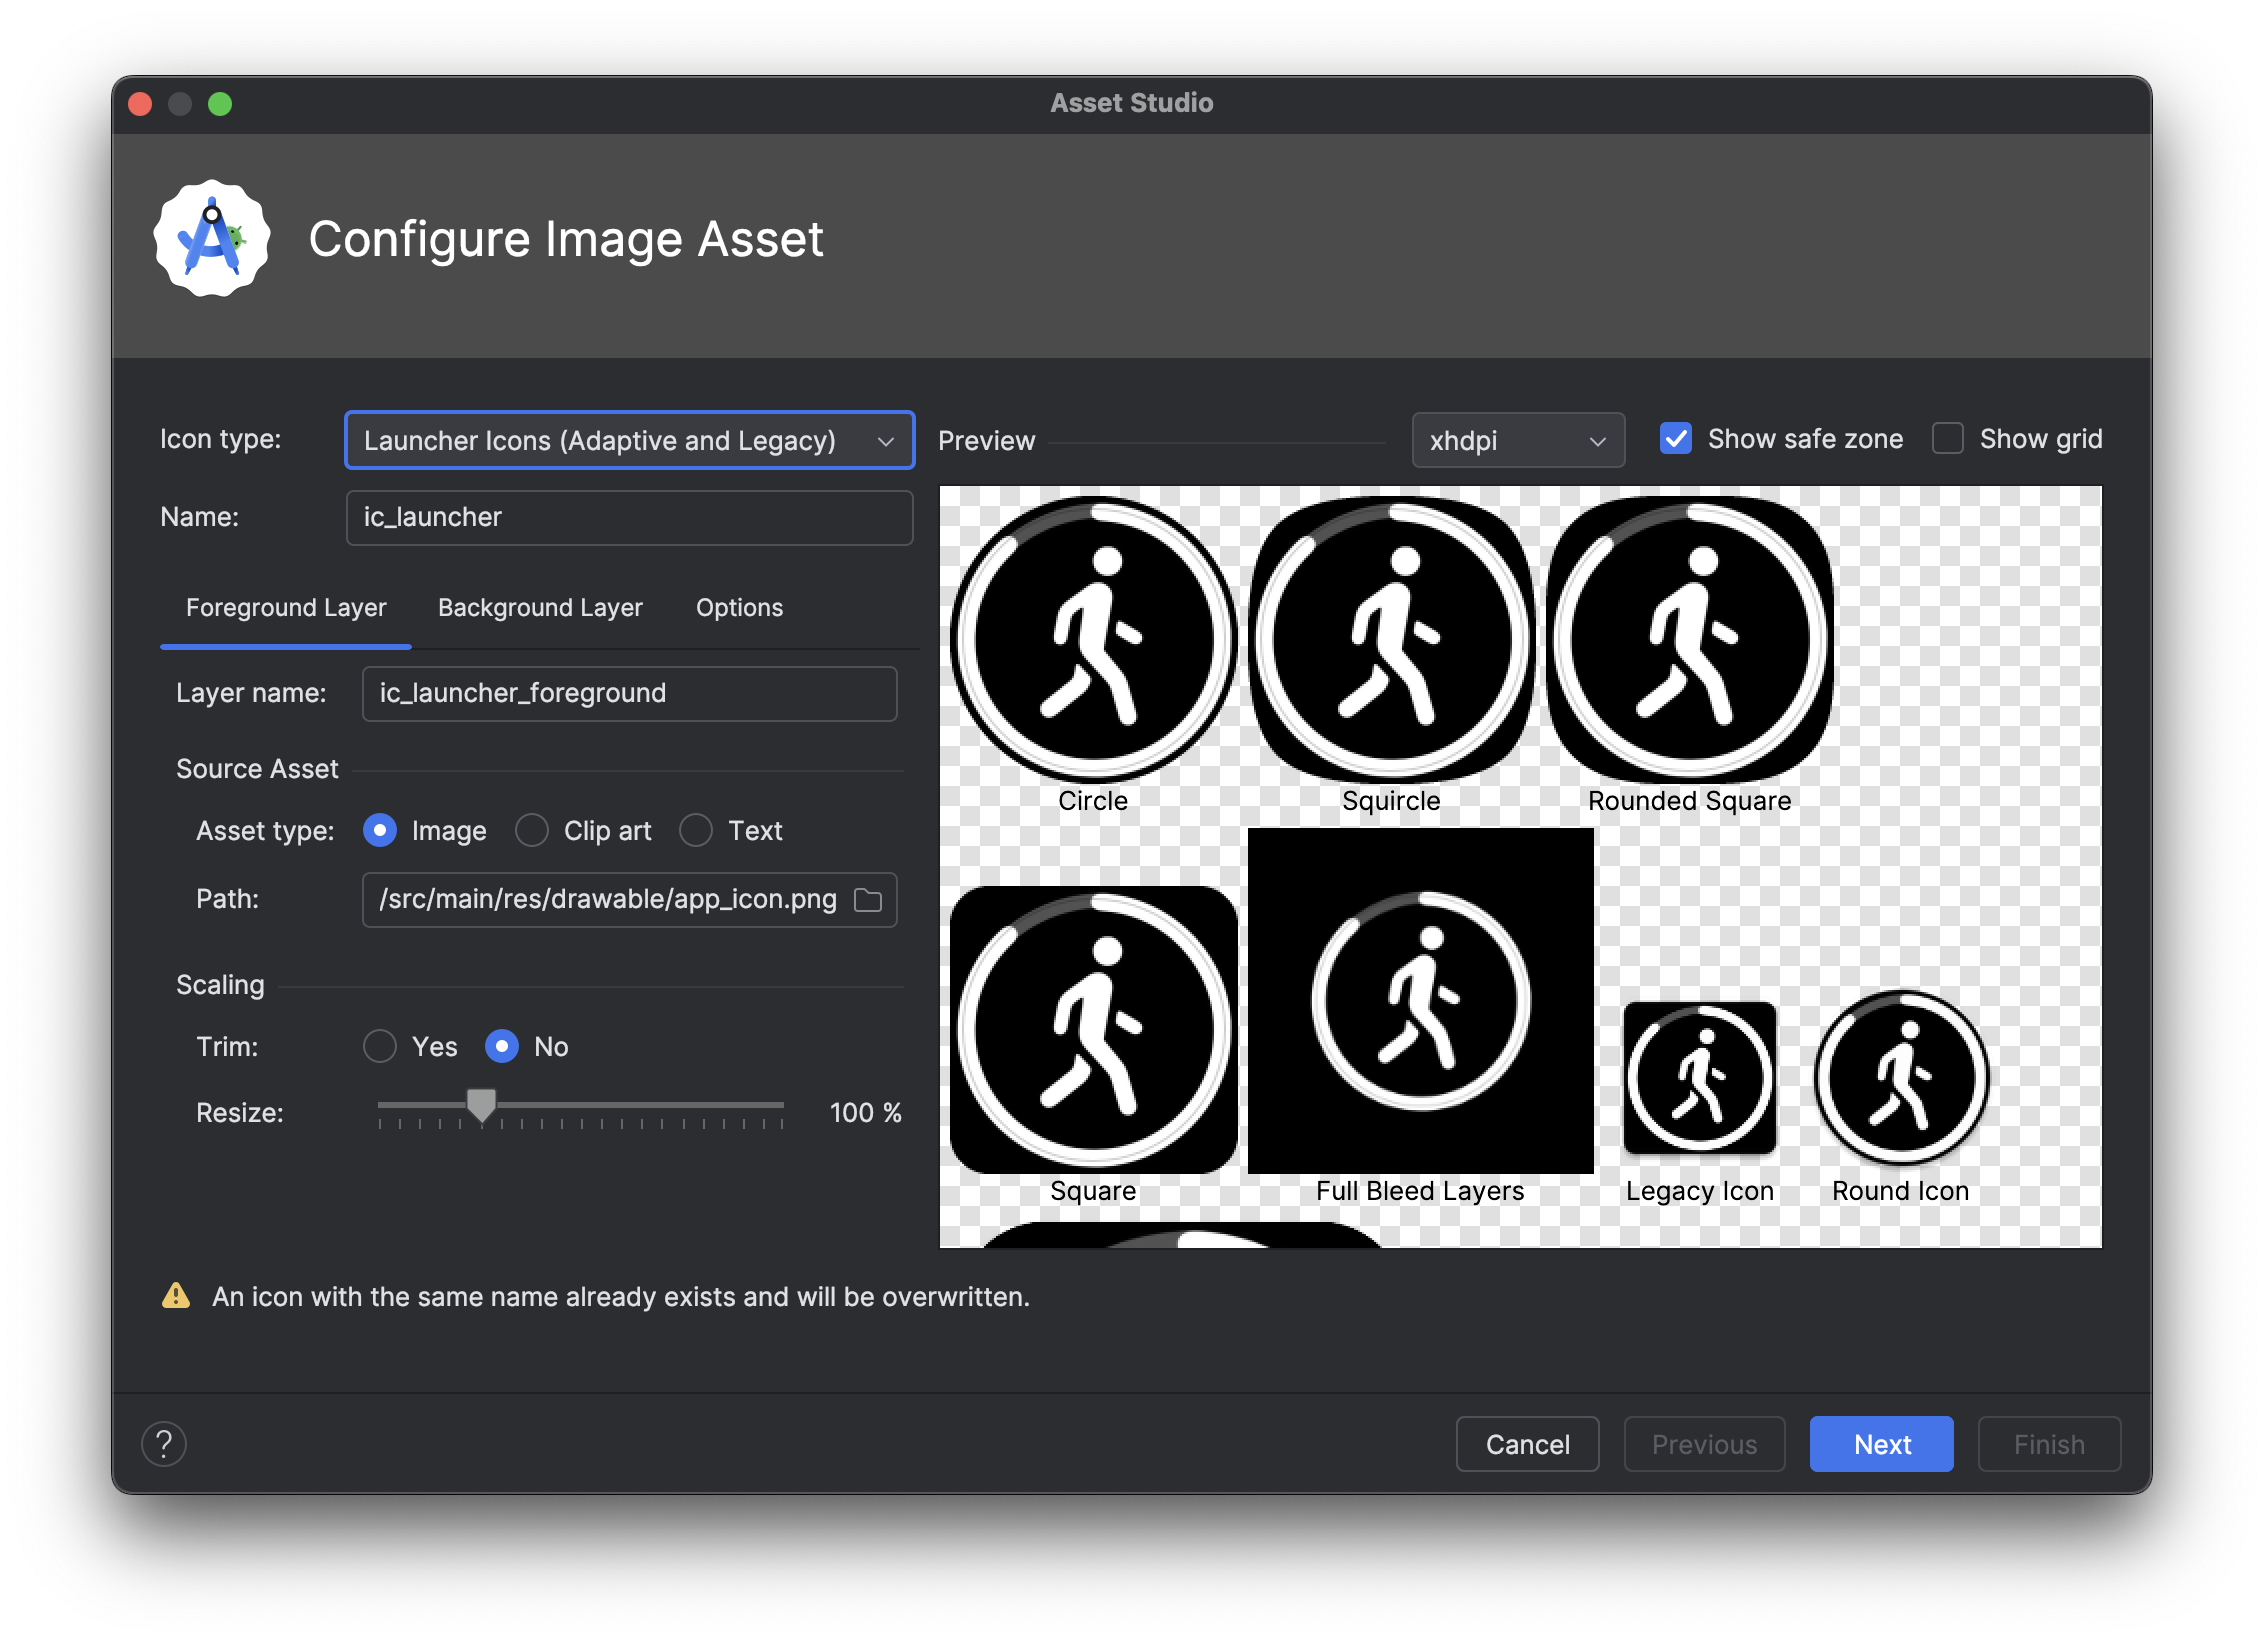
\includegraphics[width=0.5\textwidth]{res/img/appIcon.png}
            \caption{Generating Icons in Android Studio}
            \label{fig:ex2_1.1}
        \end{figure}
        
        Android Studio handled the generation of all necessary formats for the image, including various resolution sizes and shapes (see Figure~\ref{fig:ex2_2.2}).
        
        \begin{figure}[H]
            \centering
            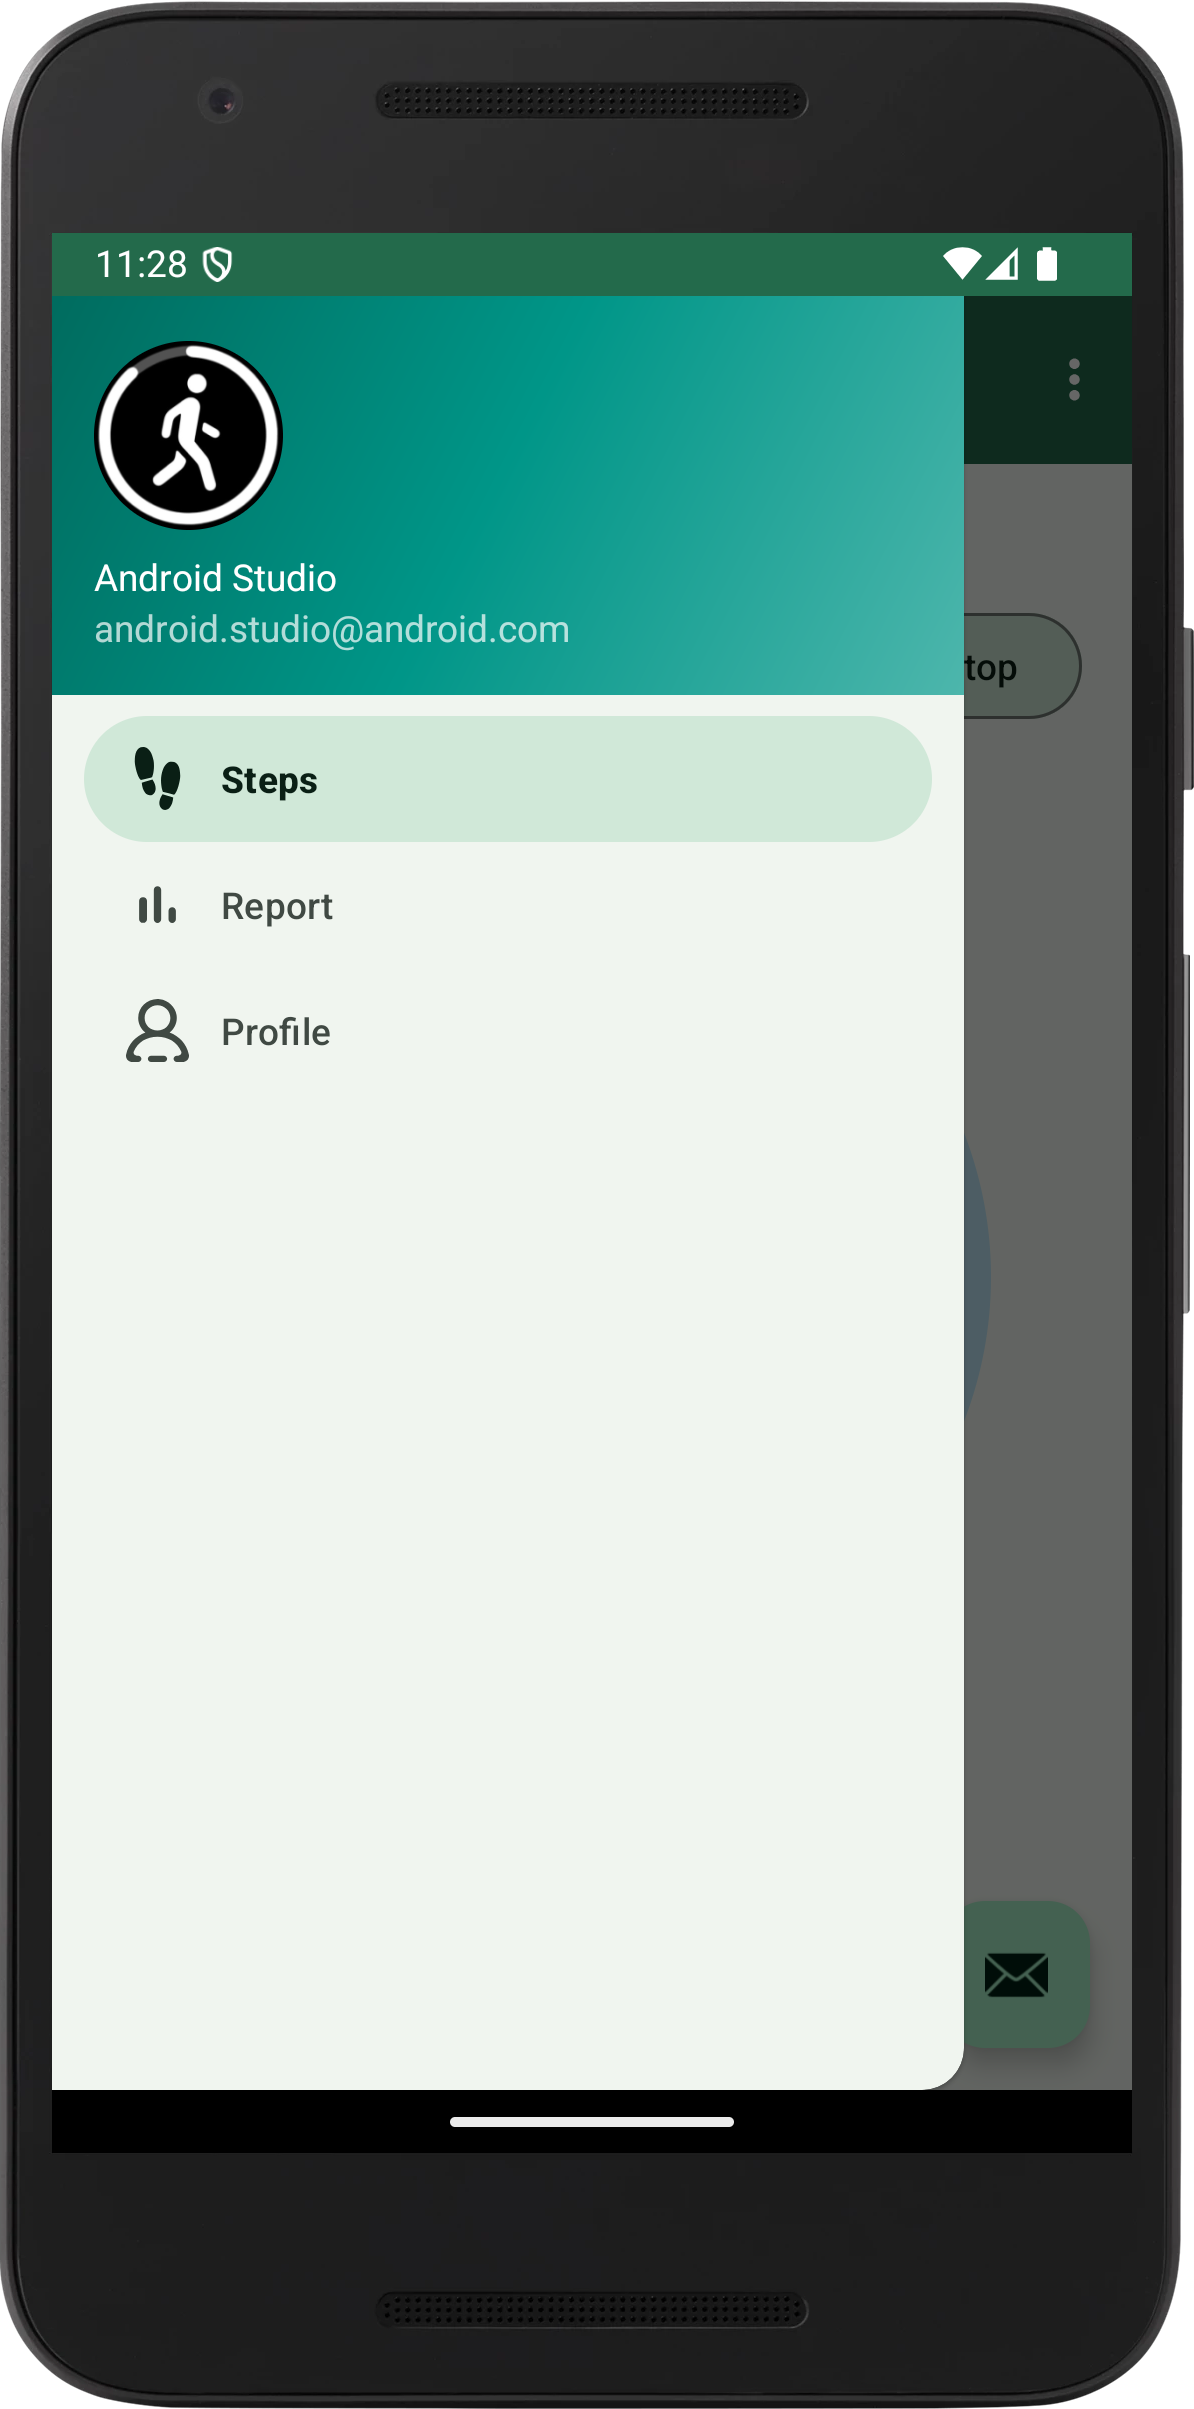
\includegraphics[width=0.20\textwidth]{res/img/icon1.png}
            \hspace{0.05\textwidth}
            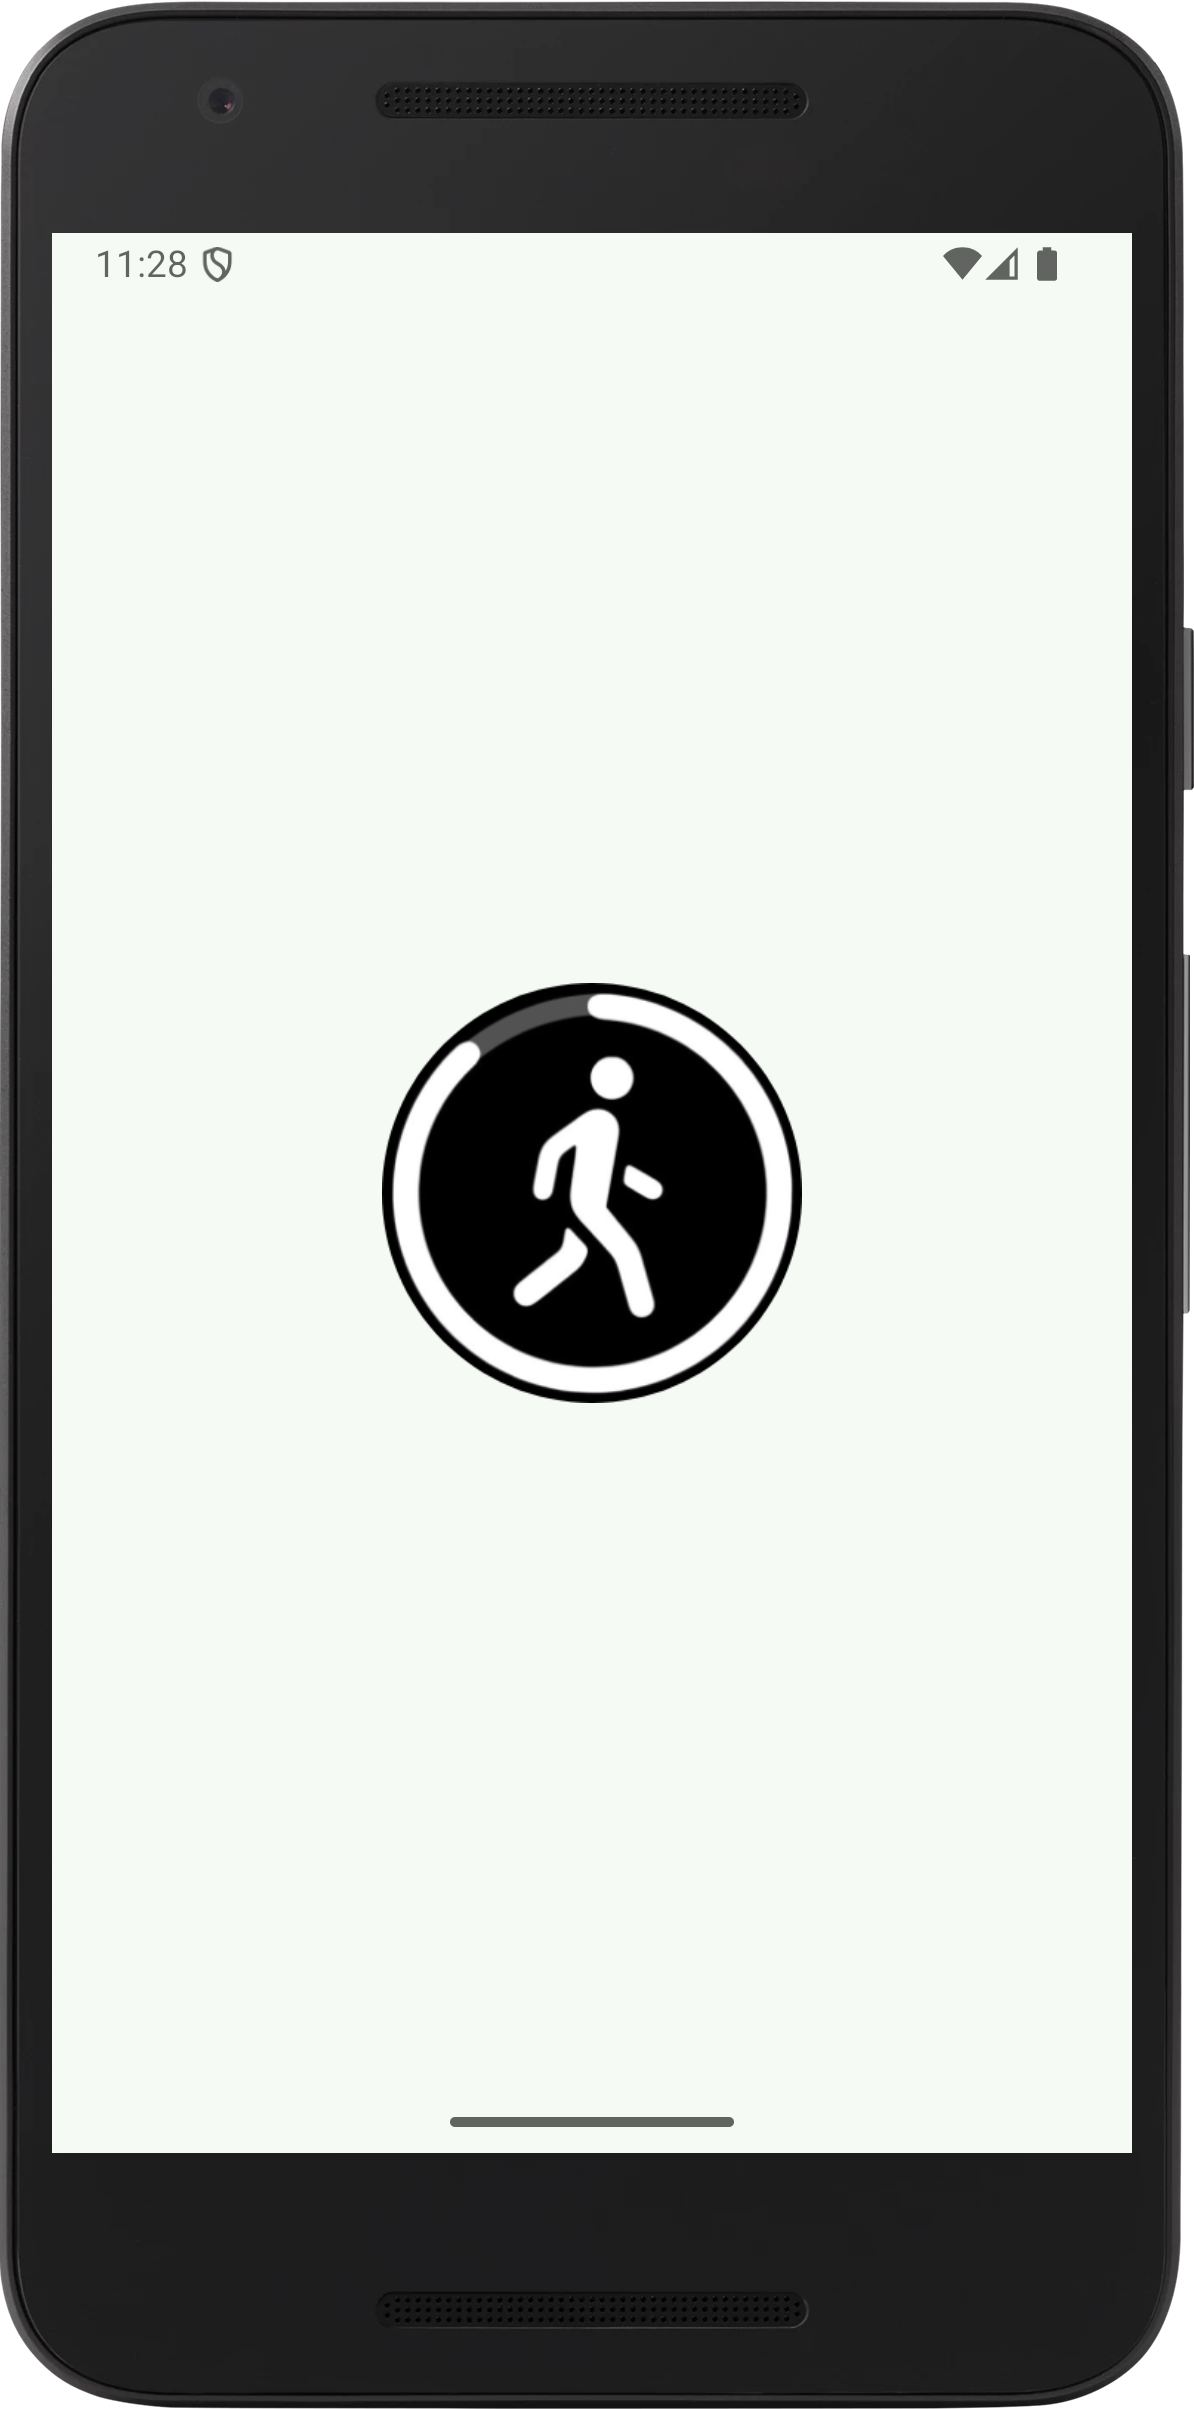
\includegraphics[width=0.20\textwidth]{res/img/icon2.png}      
            \hspace{0.05\textwidth}
            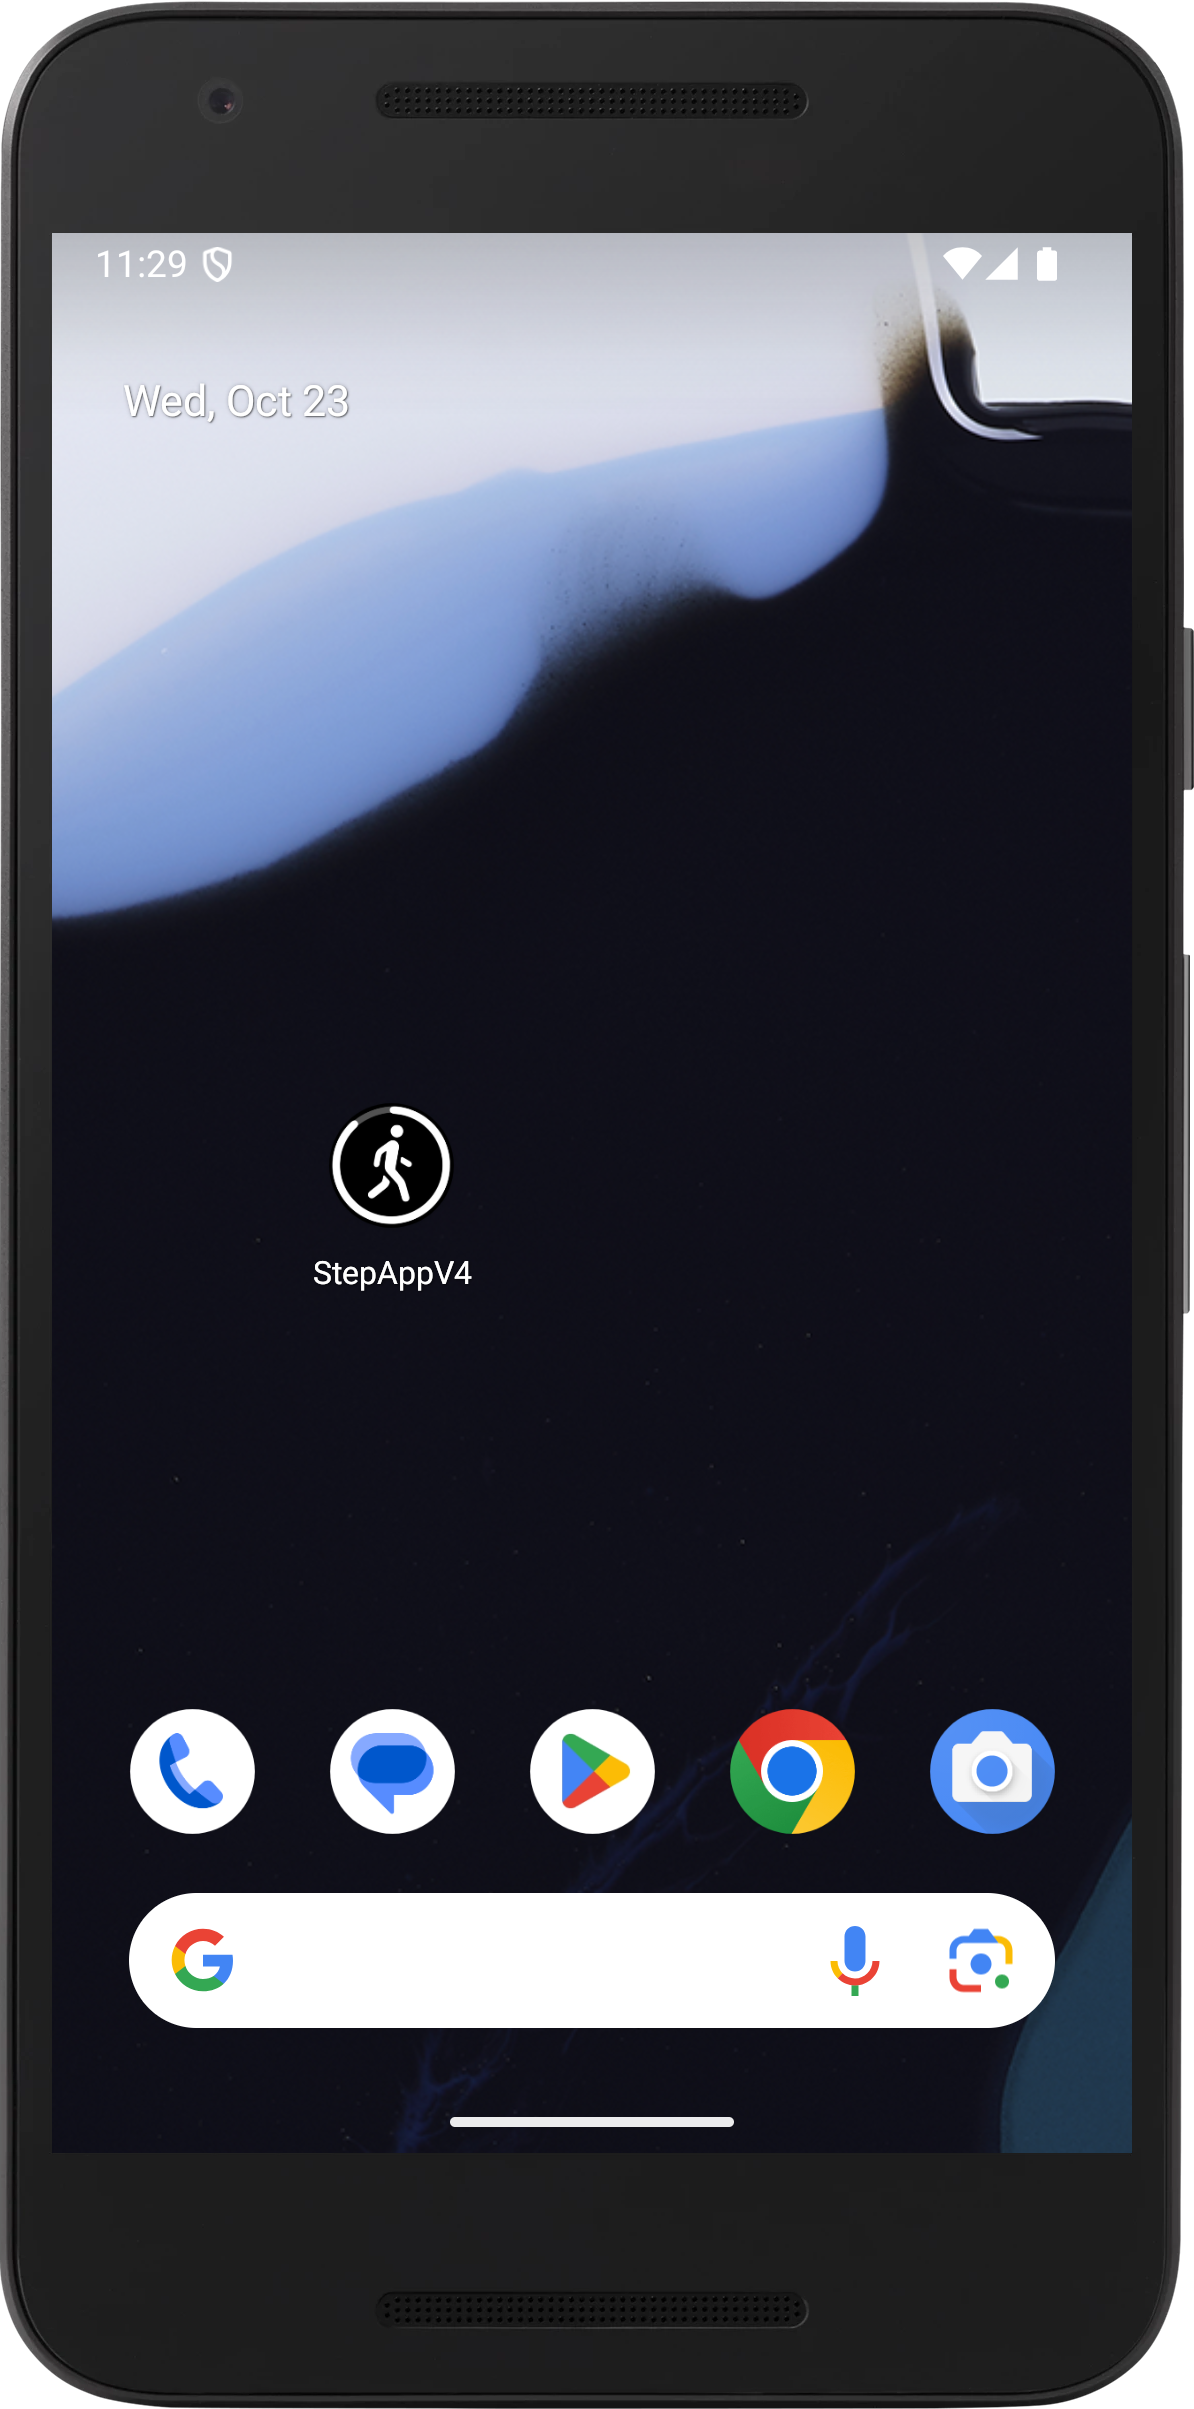
\includegraphics[width=0.20\textwidth]{res/img/icon3.png}
            \caption{Generated Icons with Different Resolutions and Shapes}
            \label{fig:ex2_2.2}
        \end{figure}



\newpage


\subsection{Implement Dark Theme}
    To implement the dark theme, I utilized the \texttt{AppCompatDelegate} class provided by Android's support library. This allows for easy switching between light and dark modes. The dark mode can be toggled by the user via a switch placed in the \texttt{Profile} page (see Figure~\ref{fig:ex2_3}).

    \begin{figure}[H]
        \centering
        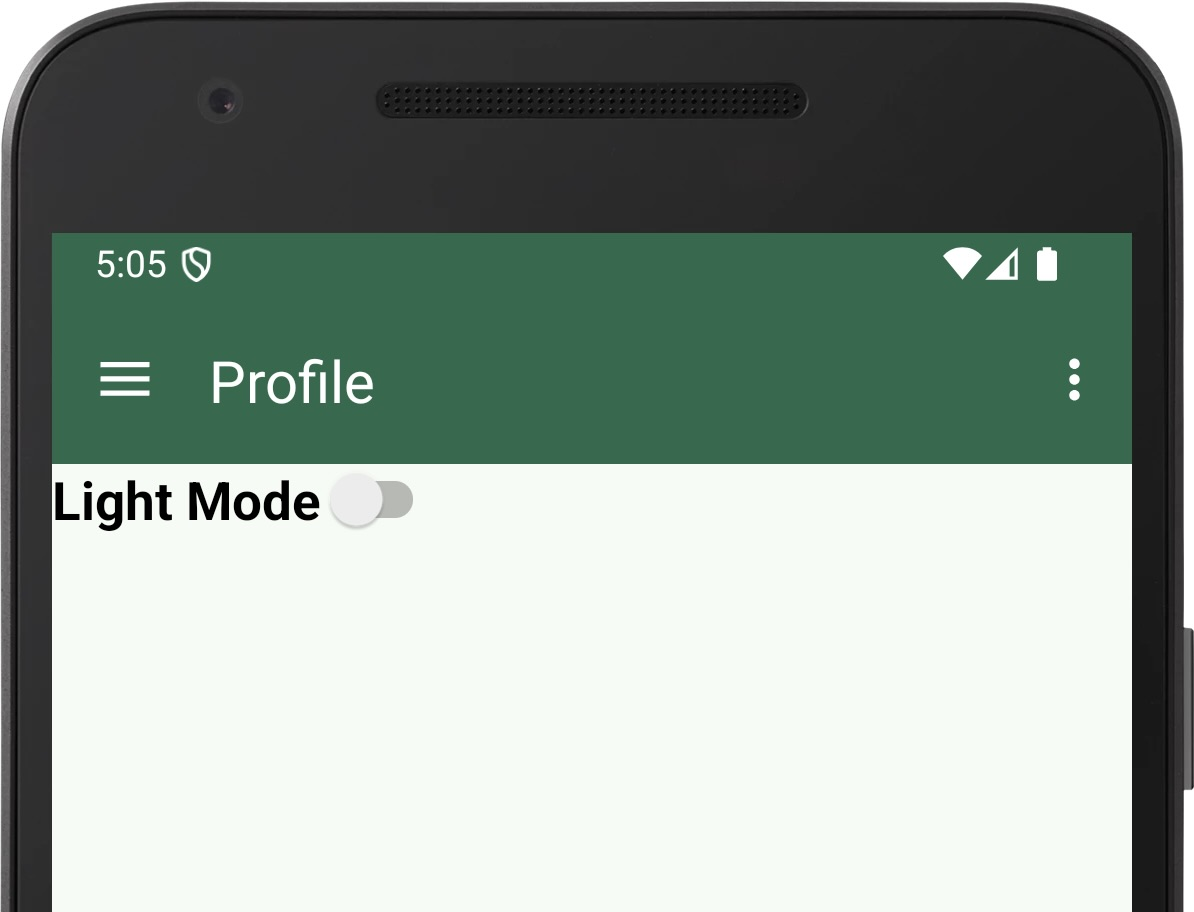
\includegraphics[width=0.2\textwidth]{res/img/dark_theme_switch.png}
        \caption{Switch for toggling between Light and Dark Modes}
        \label{fig:ex2_3}
    \end{figure}

    The dark mode implementation involved modifying the \texttt{ProfileFragment} and adding an \\ \texttt{OnCheckedChangeListener} to the switch. Depending on whether the switch is checked or not, the theme is switched using \texttt{AppCompatDelegate.setDefaultNightMode()}. If the switch is turned on, the dark theme is enabled using \texttt{AppCompatDelegate.MODE\_NIGHT\_YES}, and if the switch is off, the light theme is restored using \texttt{AppCompatDelegate.MODE\_NIGHT\_NO}.

    The relevant code for the theme switching logic is shown below:

    \lstinputlisting[firstline=45]{../app/src/main/java/com/example/stepappv4/ui/slideshow/ProfileFragment.java}

    Additionally, I ensured that the \texttt{colors.xml} file contained separate color definitions for both light and dark modes . This file is located in the \texttt{res/values} and \texttt{res/values-night} directories for light and dark modes, respectively. Same thing I had to do for the Themes, this prevented the app from changing layout changes. The following figures are some screenshots of the app in dark mode (see Figure~\ref{fig:ex2_2.4}).

    \begin{figure}[H]
        \centering
        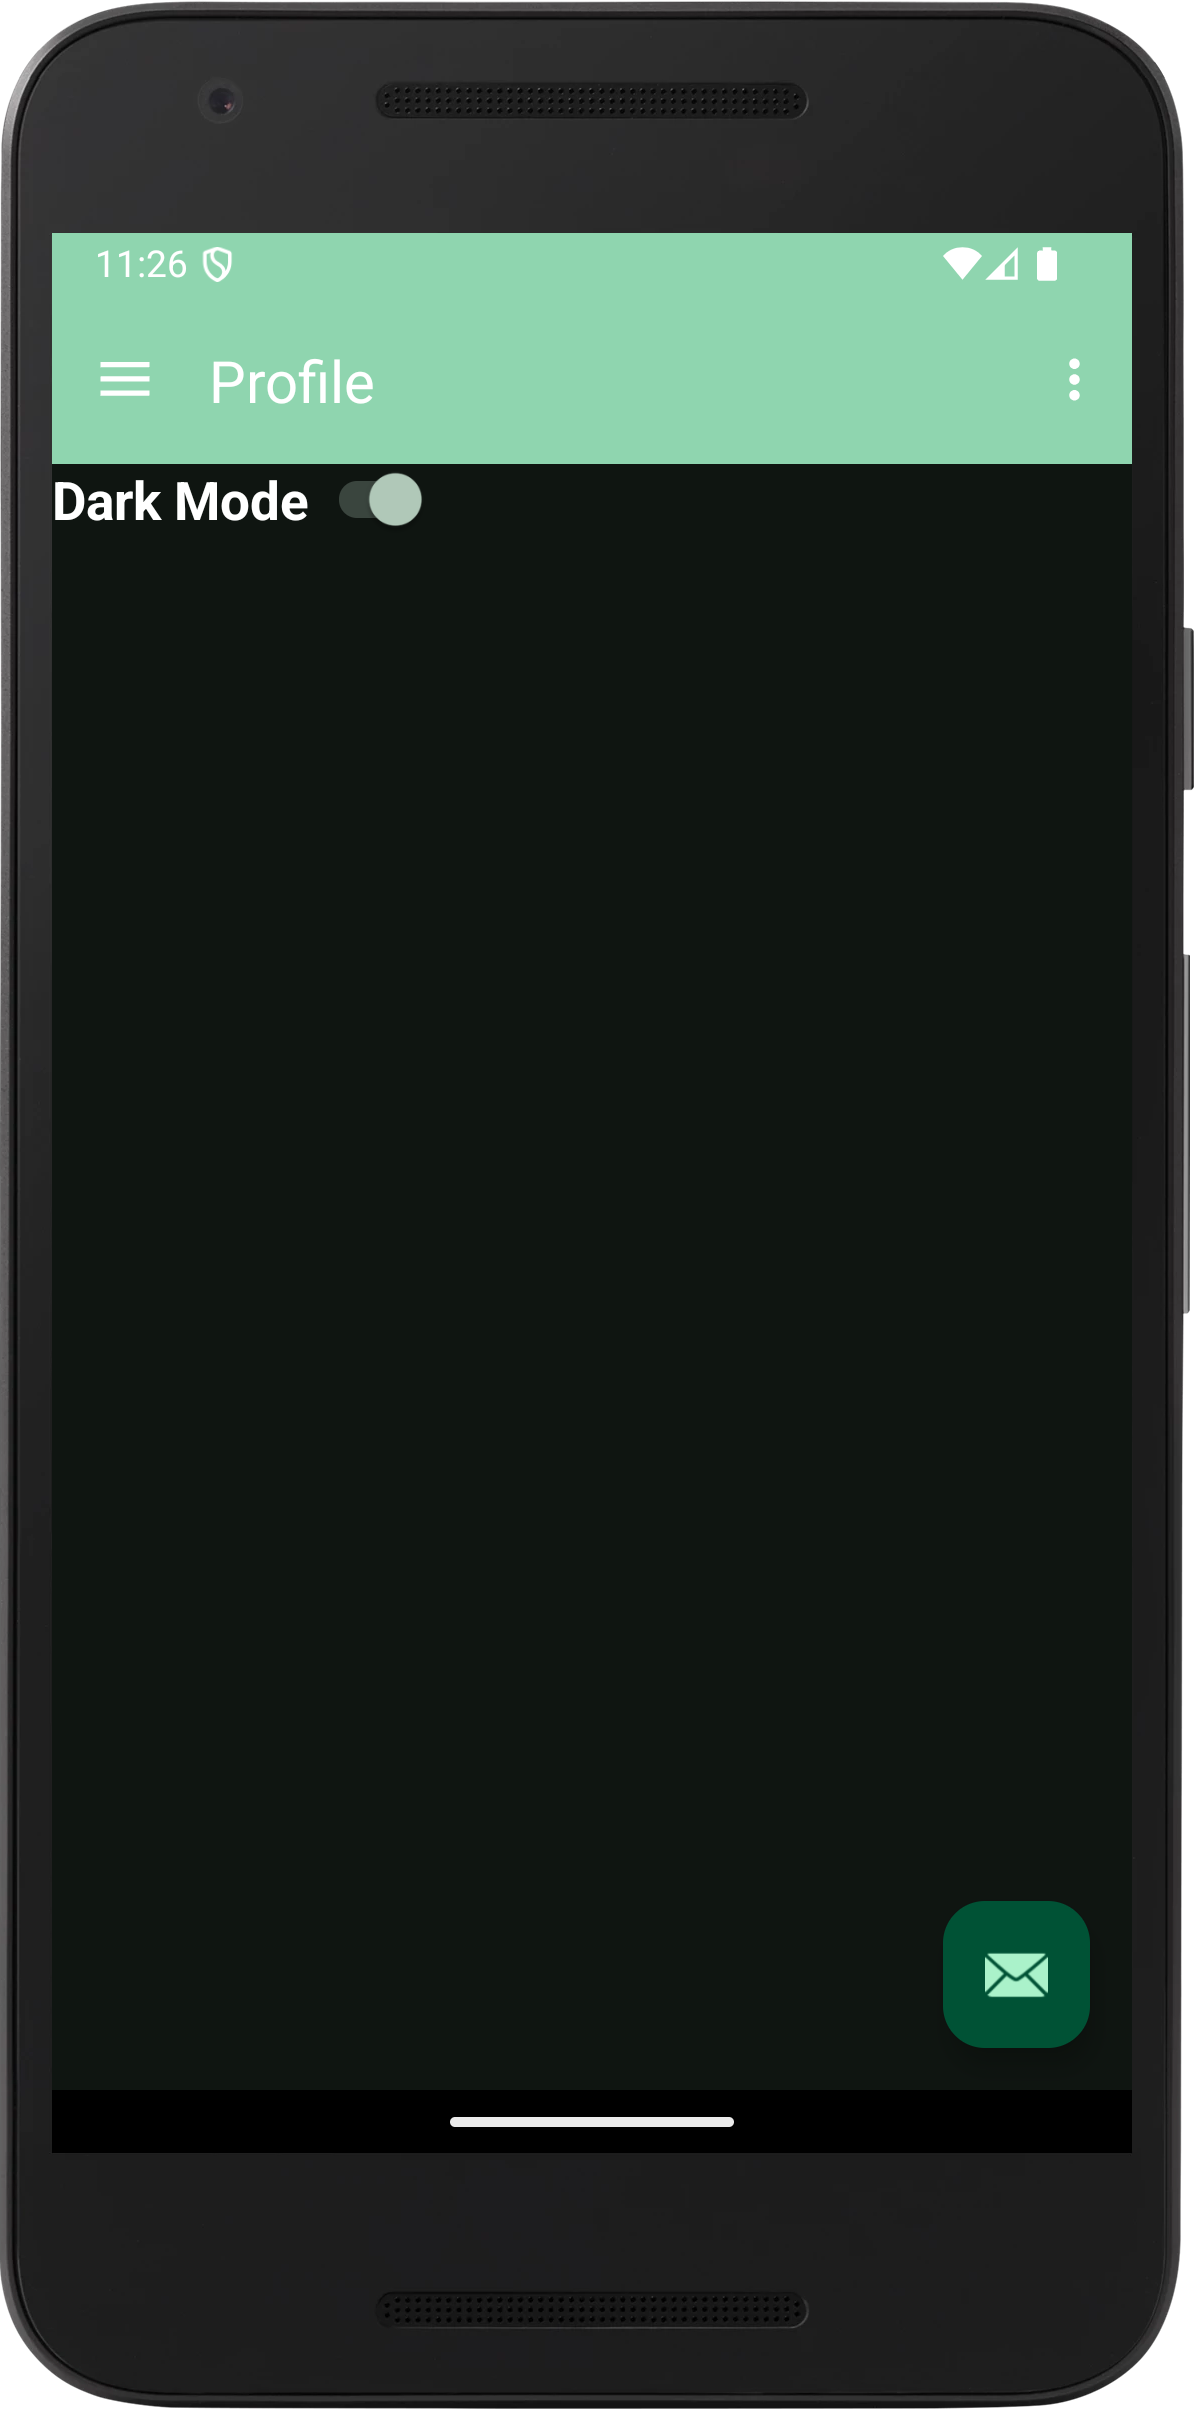
\includegraphics[width=0.20\textwidth]{res/img/darkMode1.png}
        \hspace{0.05\textwidth}
        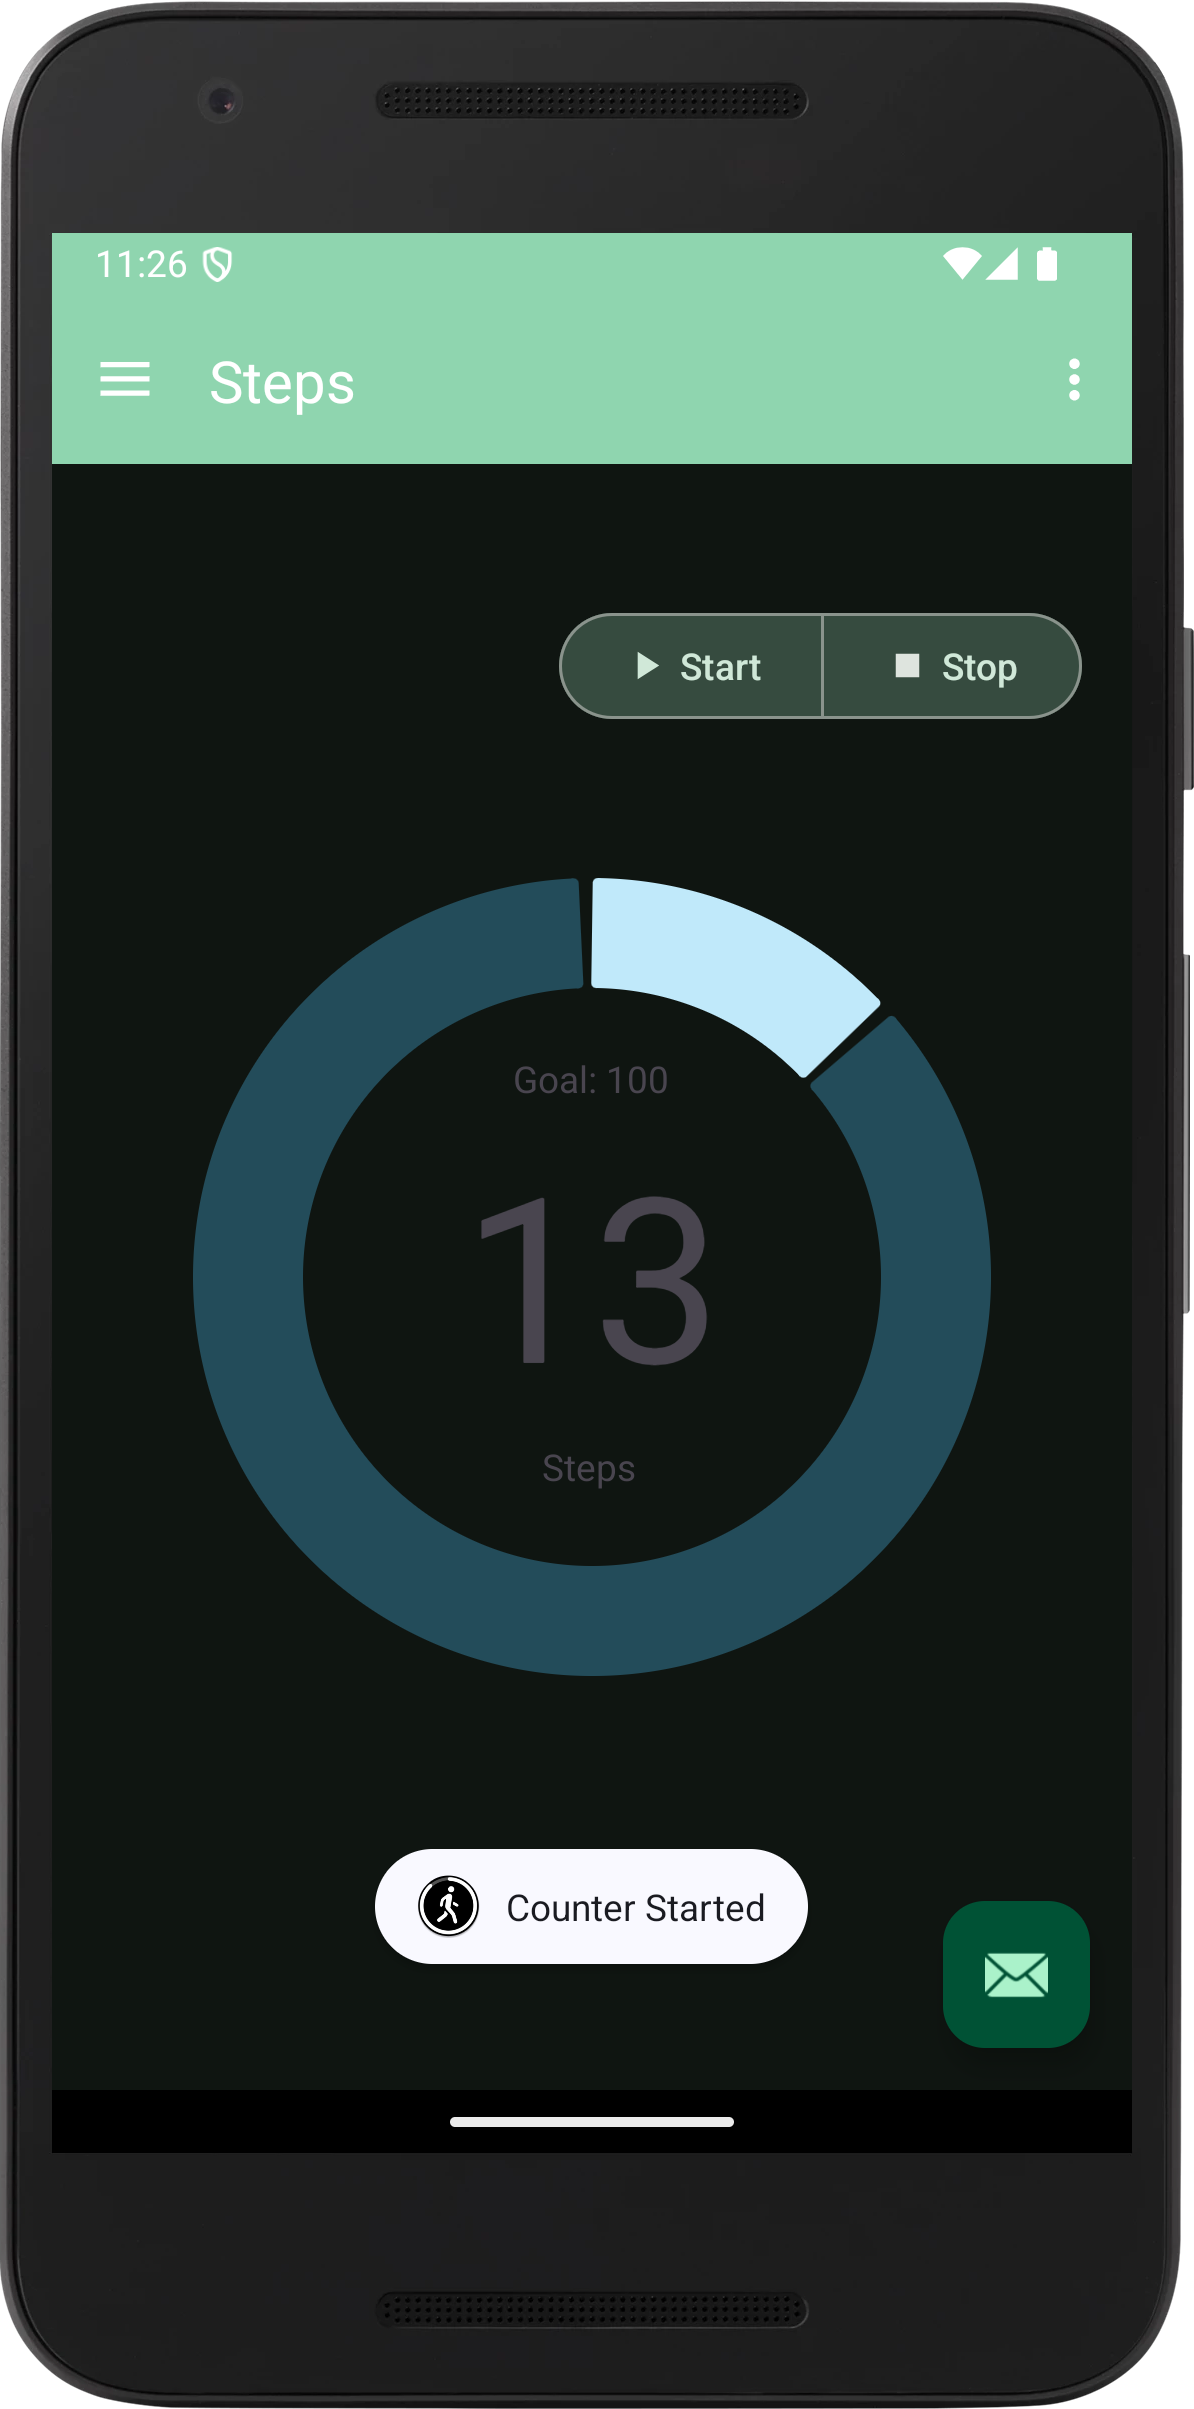
\includegraphics[width=0.20\textwidth]{res/img/darkMode2.png}      
        \hspace{0.05\textwidth}
        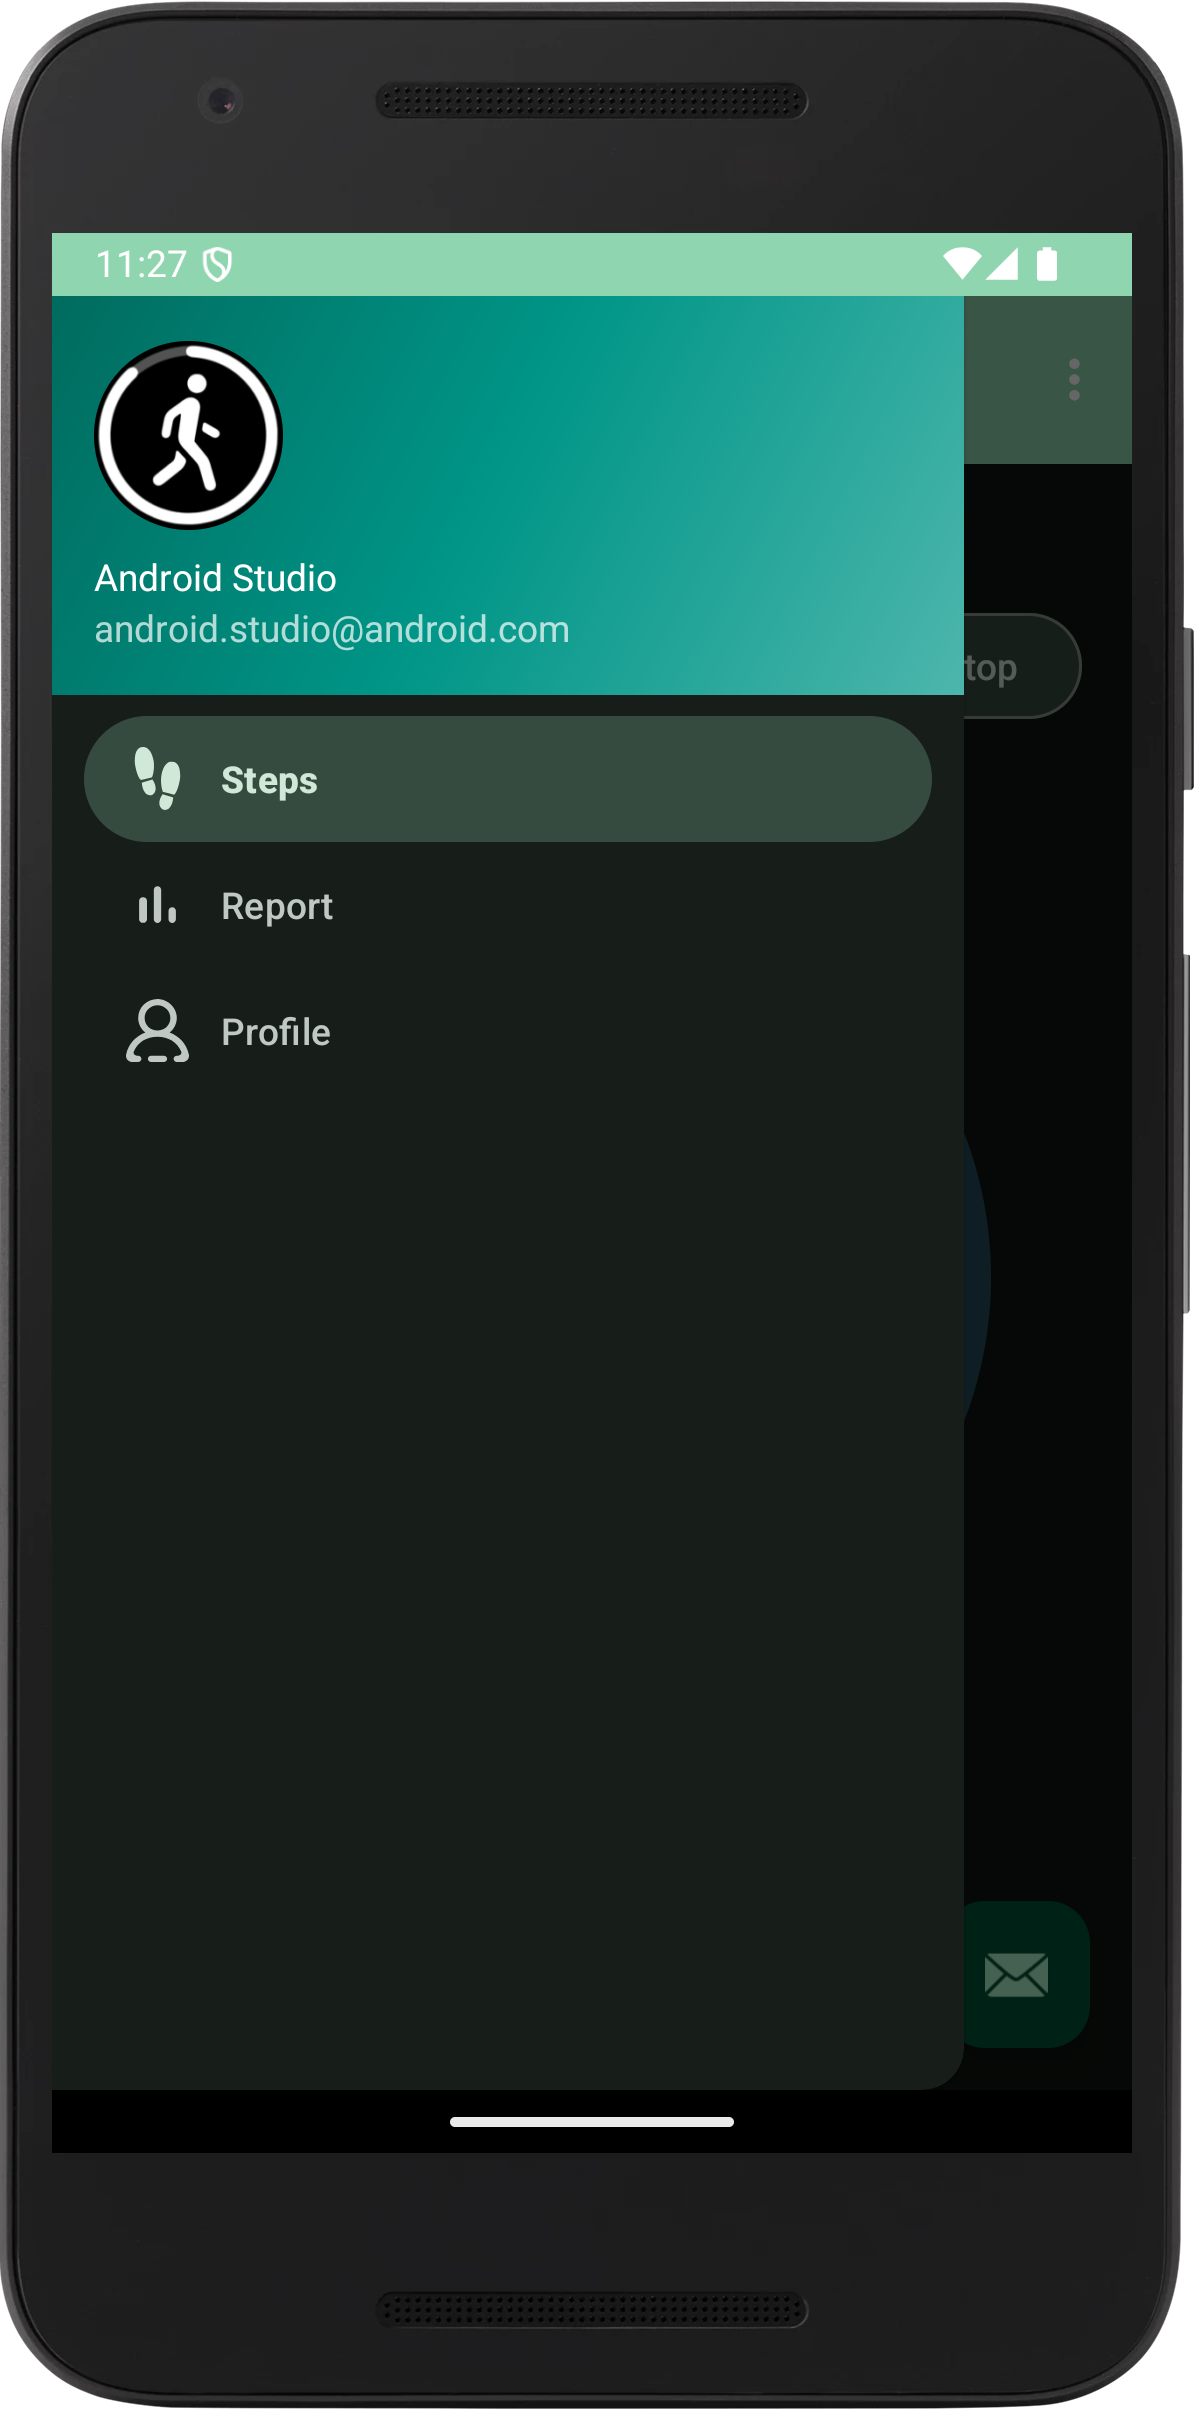
\includegraphics[width=0.20\textwidth]{res/img/darkMode3.png}
        \caption{Generated Icons with Different Resolutions and Shapes}
        \label{fig:ex2_2.4}
    \end{figure}

\newpage
\section{Exercise 3 – Step Counter}

\subsection{Android STEP\_DETECTOR}

First of all I modified the variable \texttt{accSensor} in the \texttt{StepsFragment} class to be of type:\\ \texttt{Sensor.TYPE\_STEP\_DETECTOR}. I could have easly have defined another variable but I wanted to make sure that all the counts were updted thanks to this sensor and not the previsouly used\\ \texttt{Sensor.TYP\_LINEAR\_ACCELERATION}.

\begin{verbatim}
    accSensor = sensorManager.getDefaultSensor(Sensor.TYPE_STEP_DETECTOR);
\end{verbatim}

Then I moved to the \texttt{StepCounterListener} class and mofied the \texttt{onSensorChanged} method to call the \texttt{countSteps} method. 

\lstinputlisting[
    firstline=101, 
    lastline=103, 
    firstnumber=101,
    caption=\texttt{\codepath/StepCounterListener.java}
]{\codepath/StepCounterListener.java}

\lstinputlisting[
    firstline=150, 
    lastline=161, 
    firstnumber=150,
    caption=\texttt{\codepath/StepCounterListener.java}
]{\codepath/StepCounterListener.java}

This method is used to update the step count, the step count text view and the step count progress bar (for the )

\end{document}